\documentclass[a4paper,12pt]{article}

\usepackage{graphicx}
\usepackage{caption}
\usepackage{subcaption}
\usepackage{tikz}
\usepackage{pgf}
\usepackage{amsmath}
\usepackage{amssymb}
\usetikzlibrary{arrows.meta}
\usepackage[utf8]{inputenc}
\usepackage[english,greek]{babel}
\usepackage{hyperref}

\title{Προσομοίωση και Μοντελοποίηση \newline Δυναμικών Συστημάτων \newline 
\selectlanguage{english}Project\selectlanguage{greek}}
\author{Ρουσομάνης Γεώργιος (ΑΕΜ: 10703)}
\date{Ιούνιος 2025}

\begin{document}

\maketitle

\section*{Εισαγωγή}

\section*{Θέμα 1}

Σε αυτό το μέρος μελετάται ένα γραμμικό δυναμικό σύστημα δεύτερης τάξης της μορφής:
\begin{equation}
\dot{x}(t) = A x(t) + B u(t),
\end{equation}
όπου $x(t) \in \mathbb{R}^2$ είναι το διάνυσμα των καταστάσεων, και $u(t) \in \mathbb{R}$ 
η είσοδος του συστήματος. Οι πίνακες $A \in \mathbb{R}^{2 \times 2}$ και 
$B \in \mathbb{R}^{2 \times 1}$ είναι άγνωστοι αλλά σταθεροί. Επίσης, γνωρίζουμε ότι:
\[
-3 \leq a_{11} \leq -1, \quad \text{και} \quad b_2 \geq 1.
\]

Σκοπός είναι η ανάπτυξη και ανάλυση ενός αλγορίθμου πραγματικού χρόνου για την εκτίμηση  
$\hat{A},\,\hat{B}$ των πινάκων $A$ και $B$, με δεδομένο ότι τόσο η είσοδος $u(t)$ όσο και  
οι καταστάσεις $x(t)$ είναι μετρήσιμες. Για τη σχεδίαση του αλγορίθμου, αρχικά υποθέτουμε ότι  
δεν υπάρχουν διαταραχές στις μετρήσεις των καταστάσεων του συστήματος. Στη συνέχεια,  
εισάγεται στο σύστημα σφάλμα πόλωσης και επανασχεδιάζεται ο αλγόριθμος, με στόχο  
τη μελέτη της επίδρασης του σφάλματος στην ακρίβεια των εκτιμήσεων. Για σκοπούς προσομοίωσης,  
χρησιμοποιούνται ως πραγματικές τιμές οι παρακάτω πίνακες:
\[
A = 
\begin{bmatrix}
-2.15 & 0.25 \\
-0.75 & -2
\end{bmatrix}, \quad
B = 
\begin{bmatrix}
0 \\
1.5
\end{bmatrix}.
\]

\subsection*{Εκτίμηση Παραμέτρων χωρίς Σφάλμα Πόλωσης}

Πρωτού προχωρήσουμε στη σχεδίαση του αλγορίθμου πραγματικού χρόνου για την εκτίμηση των $A,\,B$,  
πρέπει να επιλέξουμε το είδος της εισόδου που θα εφαρμόσουμε στο σύστημα, καθώς και τη συχνότητα  
δειγματοληψίας. Μία συνήθης πρακτική για την επιλογή της συχνότητας δειγματοληψίας είναι να την  
ορίζουμε περίπου δέκα φορές μεγαλύτερη από το εύρος ζώνης του συστήματος. Ωστόσο, επειδή το μοντέλο  
μας υπάγεται στην κατηγορία "γκρι κουτί", η εκ των προτέρων γνώση μας για το σύστημα δεν επαρκεί  
για τον άμεσο υπολογισμό του εύρους ζώνης.

\subsubsection*{Επιλογή Συχνότητας Δειγματολειψίας}

Εφαρμόζουμε βηματική είσοδο στο σύστημα ώστε να εκτιμήσουμε την κυρίαρχη σταθερά χρόνου  
και να αποκτήσουμε μία πρώτη εικόνα για τη δυναμική του. Η βηματική απόκριση του συστήματος  
παρουσιάζεται στο Σχήμα~\ref{fig:task1_step_response} για συχνότητα δειγματοληψίας $f_s = 10$
\selectlanguage{english}kHz\selectlanguage{greek}. Η $f_s$ επιλέχθηκε αυθαίρετα ως μία υψηλή τιμή, 
επαρκής για να αποτυπώσει πλήρως τη δυναμική του συστήματος.

Παρατηρούμε ότι η έξοδος $x_2(t)$ αντιστοιχεί είτε σε κρίσιμα αποσβεννύμενο σύστημα ($\zeta = 1$)  
είτε σε υποαποσβεννύμενη ταλάντωση ($0 < \zeta < 1$) με $\zeta$ πολύ κοντά στη μονάδα.  
Στην πραγματικότητα, υπάρχει μικρή υπερύψωση η οποία δεν είναι ορατή στη συγκεκριμένη κλίμακα του 
σχήματος, γεγονός που υποδηλώνει την ύπαρξη δύο συζυγών μιγαδικών πόλων.

Η μικρότερη σταθερά χρόνου $\tau$ αντιστοιχεί στην $x_2(t)$, η οποία παρουσιάζει ταχύτερη  
απόκριση. Από το διάγραμμα εκτιμάται ως $\tau \approx 2$. Συνεπώς, η συχνότητα δειγματοληψίας  
πρέπει να ικανοποιεί $f_s > 10/\tau$.

Για το πραγματικό σύστημα, οι ιδιοτιμές του πίνακα $A$ είναι $\lambda_{1,2} = -2.075 \pm 0.4265j$, 
ο συντελεστής απόσβεσης είναι $\zeta = 0.98$, και η σταθερά χρόνου
$\tau = \frac{1}{\zeta \omega_n} = 2.075$, πολύ κοντά στην αρχική μας εκτίμηση.

\begin{figure}
    \centering
    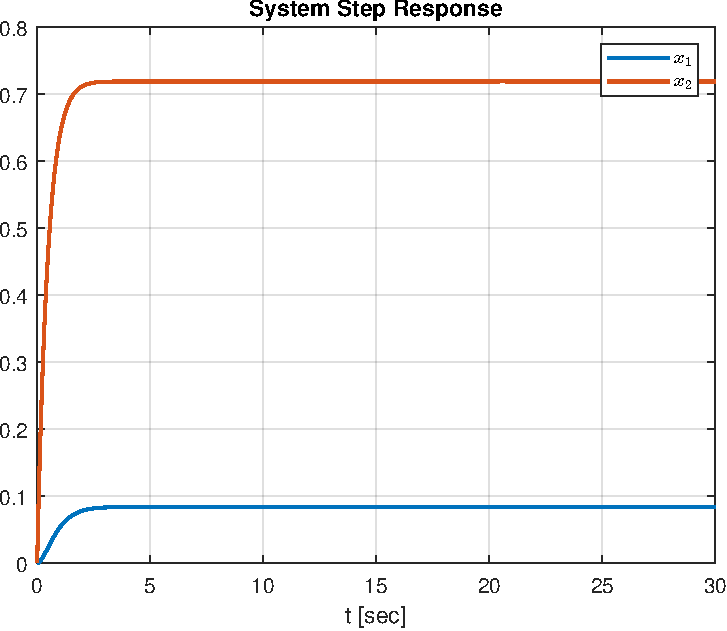
\includegraphics[width=0.75\linewidth]{plot/task1_step_response.pdf}
    \caption{Βηματική απόκριση του συστήματος}
    \label{fig:task1_step_response}
\end{figure}

\subsubsection*{Επιλογή Αλγορίθμου Πραγματικού Χρόνου}
Λόγω της εκ των προτέρων γνώσης που έχουμε για το επιτρεπτό εύρος τιμών ορισμένων παραμέτρων, 
ο χώρος αναζήτησης $\Theta$ των παραμέτρων του μοντέλου θα είναι ένα υποσύνολο του $\mathbb{R}^n$.
Θα χρησιμοποιήσουμε κάποιο αναδρομικό αλγόριθμο προβολής ο οποίος εξασφαλίζει ότι οι εκτιμήσεις των
παραμέτρων παραμένουν εντός του $\Theta$. Ειδικότερα θα χρησιμοποιήσουμε τη μέθοδο 
\selectlanguage{english}Lyapunov\selectlanguage{greek} με προβολή.

Πρωτού προχωρήσουμε στην εκτίμηση των παραμέτρων, θα εξετάσουμε την ευστάθεια της μεθόδου 
\selectlanguage{english}Lyapunov\selectlanguage{greek} με Μ-δομή χωρίς προβολή. Η ανάλυσή μας
θα ισχύει και για την περίπτωση της προβολής.
Το σύστημα αναγνώρισης είναι:
\begin{equation}
    \dot{\hat{x}} = \hat{A}x + \hat{B} u + C(x - \hat{x}),
    \label{eq:lyapunov_mixed_identification_system}
\end{equation}
όπου $C$ συμμετρικός και θετικά ημιορισμένος πίνακας. Η παράγωγος του σφάλματος αναγνώρισης $e = x - \hat{x}$ 
βρίσκεται:
\begin{equation}
    \dot{e} = -\tilde{A}x - \tilde{B}u - Ce
    \label{eq:lyapunov_mixed_identification_error_derivative}
\end{equation}
Η συνάρτηση \selectlanguage{english}Lyapunov\selectlanguage{greek} επιλέγεται η:
\begin{equation}
    \dot{V} = \frac{1}{2}e^{\top}e + \frac{1}{2}\mathrm{Tr}\{\tilde{A}^{\top}\tilde{A}\}
    + \frac{1}{2}\mathrm{Tr}\{\tilde{B}^{\top}\tilde{B}\}
    \label{eq:lyapunov_function}
\end{equation}
Παραγωγίζοντας την (\ref{eq:lyapunov_function}) και αντικαθιστώντας
την (\ref{eq:lyapunov_mixed_identification_error_derivative}) προκύπτει:
\begin{equation}
    \dot{V} = -e^TCe + \mathrm{Tr}\{\tilde{A}^T\dot{\hat{A}} + \tilde{B}^T\dot{\hat{B}} - 
    \tilde{A}xe^T - \tilde{B}ue^T\}.
    \label{eq:lyapunov_mixed_function_derivative_1}  
\end{equation}
Επιλέγουμε:
\begin{equation}
    \begin{aligned}
        \dot{\hat{A}} = ex^T \\ 
        \dot{\hat{B}} = eu^T
    \end{aligned}
    \label{eq:lyapunov_mixed_update_formula}
\end{equation}
και η (\ref{eq:lyapunov_mixed_function_derivative_1}) γίνεται:
\begin{equation}
    \dot{V} = -e^TCe
    \label{eq:lyapunov_mixed_function_derivative_2}
\end{equation}
Βλέπουμε ότι στη μικτή δομή ισχύει $\dot{V} \leq 0, \, \forall t$, καθώς ο $C$ είναι συμμετρικός και θετικά
ημιορισμένος. Συνεπώς, το σύστημα (\ref{eq:lyapunov_mixed_identification_system}), 
(\ref{eq:lyapunov_mixed_update_formula}) είναι ευσταθές.

Στην ανάλυσή μας θέσαμε $C = k I$, όπου $I$ είναι ο μοναδιαίος πίνακας και $k > 0$ το κέρδος. 
Η επιλογή του $k$ έγινε και πάλι με την τεχνική 
\selectlanguage{english}trial and error\selectlanguage{greek}. Μεγαλύτερες τιμές του $k$ έχουν ως 
αποτέλεσμα να υπερισχύει ο διορθωτικός όρος $C(x - \hat{x})$ στην 
(\ref{eq:lyapunov_mixed_identification_system}), οδηγώντας σε ταχύτερη σύγκλιση. Ωστόσο, πολύ μεγάλες τιμές 
του $k$ ενδέχεται να καταστήσουν το σύστημα άκαμπτο. Τελικά, επιλέγουμε $k = 5$.

\subsection*{Εκτίμηση Παραμέτρων Παρουσία Σφάλματος Πόλωσης}


\end{document}
